\documentclass[master.tex]{subfiles}
 
\newcommand{\meanxy}[1]{\left<#1\right>_{z,y}}
\newcommand{\Tflow}[0]{\overline{\Gamma}}

\begin{document}



\chapter{Polarization Equation Linearization}\label{sec:polarization_equation_evaluation}
The evaluation of the linearizations is done on a 8x128x512 8x256x1024 grid with $h_x$ and $h_y=1.0|0.5$ respectively. The following parameter set is used:
\begin{itemize}
    \item $\Delta t$: 0.025
    \item $\hat{c}$: 5.0
    \item $\hat{\epsilon}$: 27000.0
    \item $mcv$: 0.02
    \item $magnetic Shear$: 1.2
    \item $\nu_{\parallel}$: 0.11
    \item $\nu_{\perp}$: 0.11
    \item core Density: 1.5
    \item edge Density: 0.13
\end{itemize}
The simulation is run on \ac{TV} node using the GPU implementations of the \ac{SOR}-solver and gyroaveraging operator. The lower resolution grid has been run for 400.000 iterations and a state snapshot is taken every 20,000 iterations. Due to time and disk space limitations for the higher resolution only 200.000 iterations are done as well as $\Delta t$ is reduced to $0.015$ to stay in the \ac{CFL} limit.

\section{Equilibrium State}
At first the simulation develops strong turbulence and high fluctuations which result in an outburst of "material" (i. e. the total density decreases). Afterwards the simulation approaches a steady state where the properties only change little. \todo{Place Figure of Energy} This behavior can be seen by looking at the $\mathrm{E} \times \mathrm{B}$-Energy and the total density both restricted to the core-plasma (in/out separatrix). The idea now is to compare mean values over the simulation time where a equilibrium state has been reached. The errors attached to the mean values are calculated via the standard derivation but do not represent the error of multiple simulations but rather give an idea about the size of fluctuations in the equilibrium state.

\section{Evaluation}
To compare the different linearizations defined in \autoref{sec:polarization-linearizations} the mean turbulent flow in the steady state regime is compared for the core and \ac{SOL} plasma. Further on the zonal potential  $\meanxy{\phi_e}$, the zonal flow ($\partial_x \meanxy{\phi_e}$) and the vorticity also defined as zonal flow potential ($\partial_yy\meanxy{\phi_e}$) are compared.




\section{Turbulent Flow}
The turbulent flow is calculated as it is defined in \autoref{sec:simulation_quantities}. After the simulation has reached a stable regime a mean value is taken and compared. The turbulent flows for the whole simulation are displayed in \autoref{fig:turbulent-flow-low} on a semi logarithmic grid. From this figure one can already see that there is no apparent difference for the turbulent flows in regard to the lineraizations.
\begin{figure}[!htbp]
    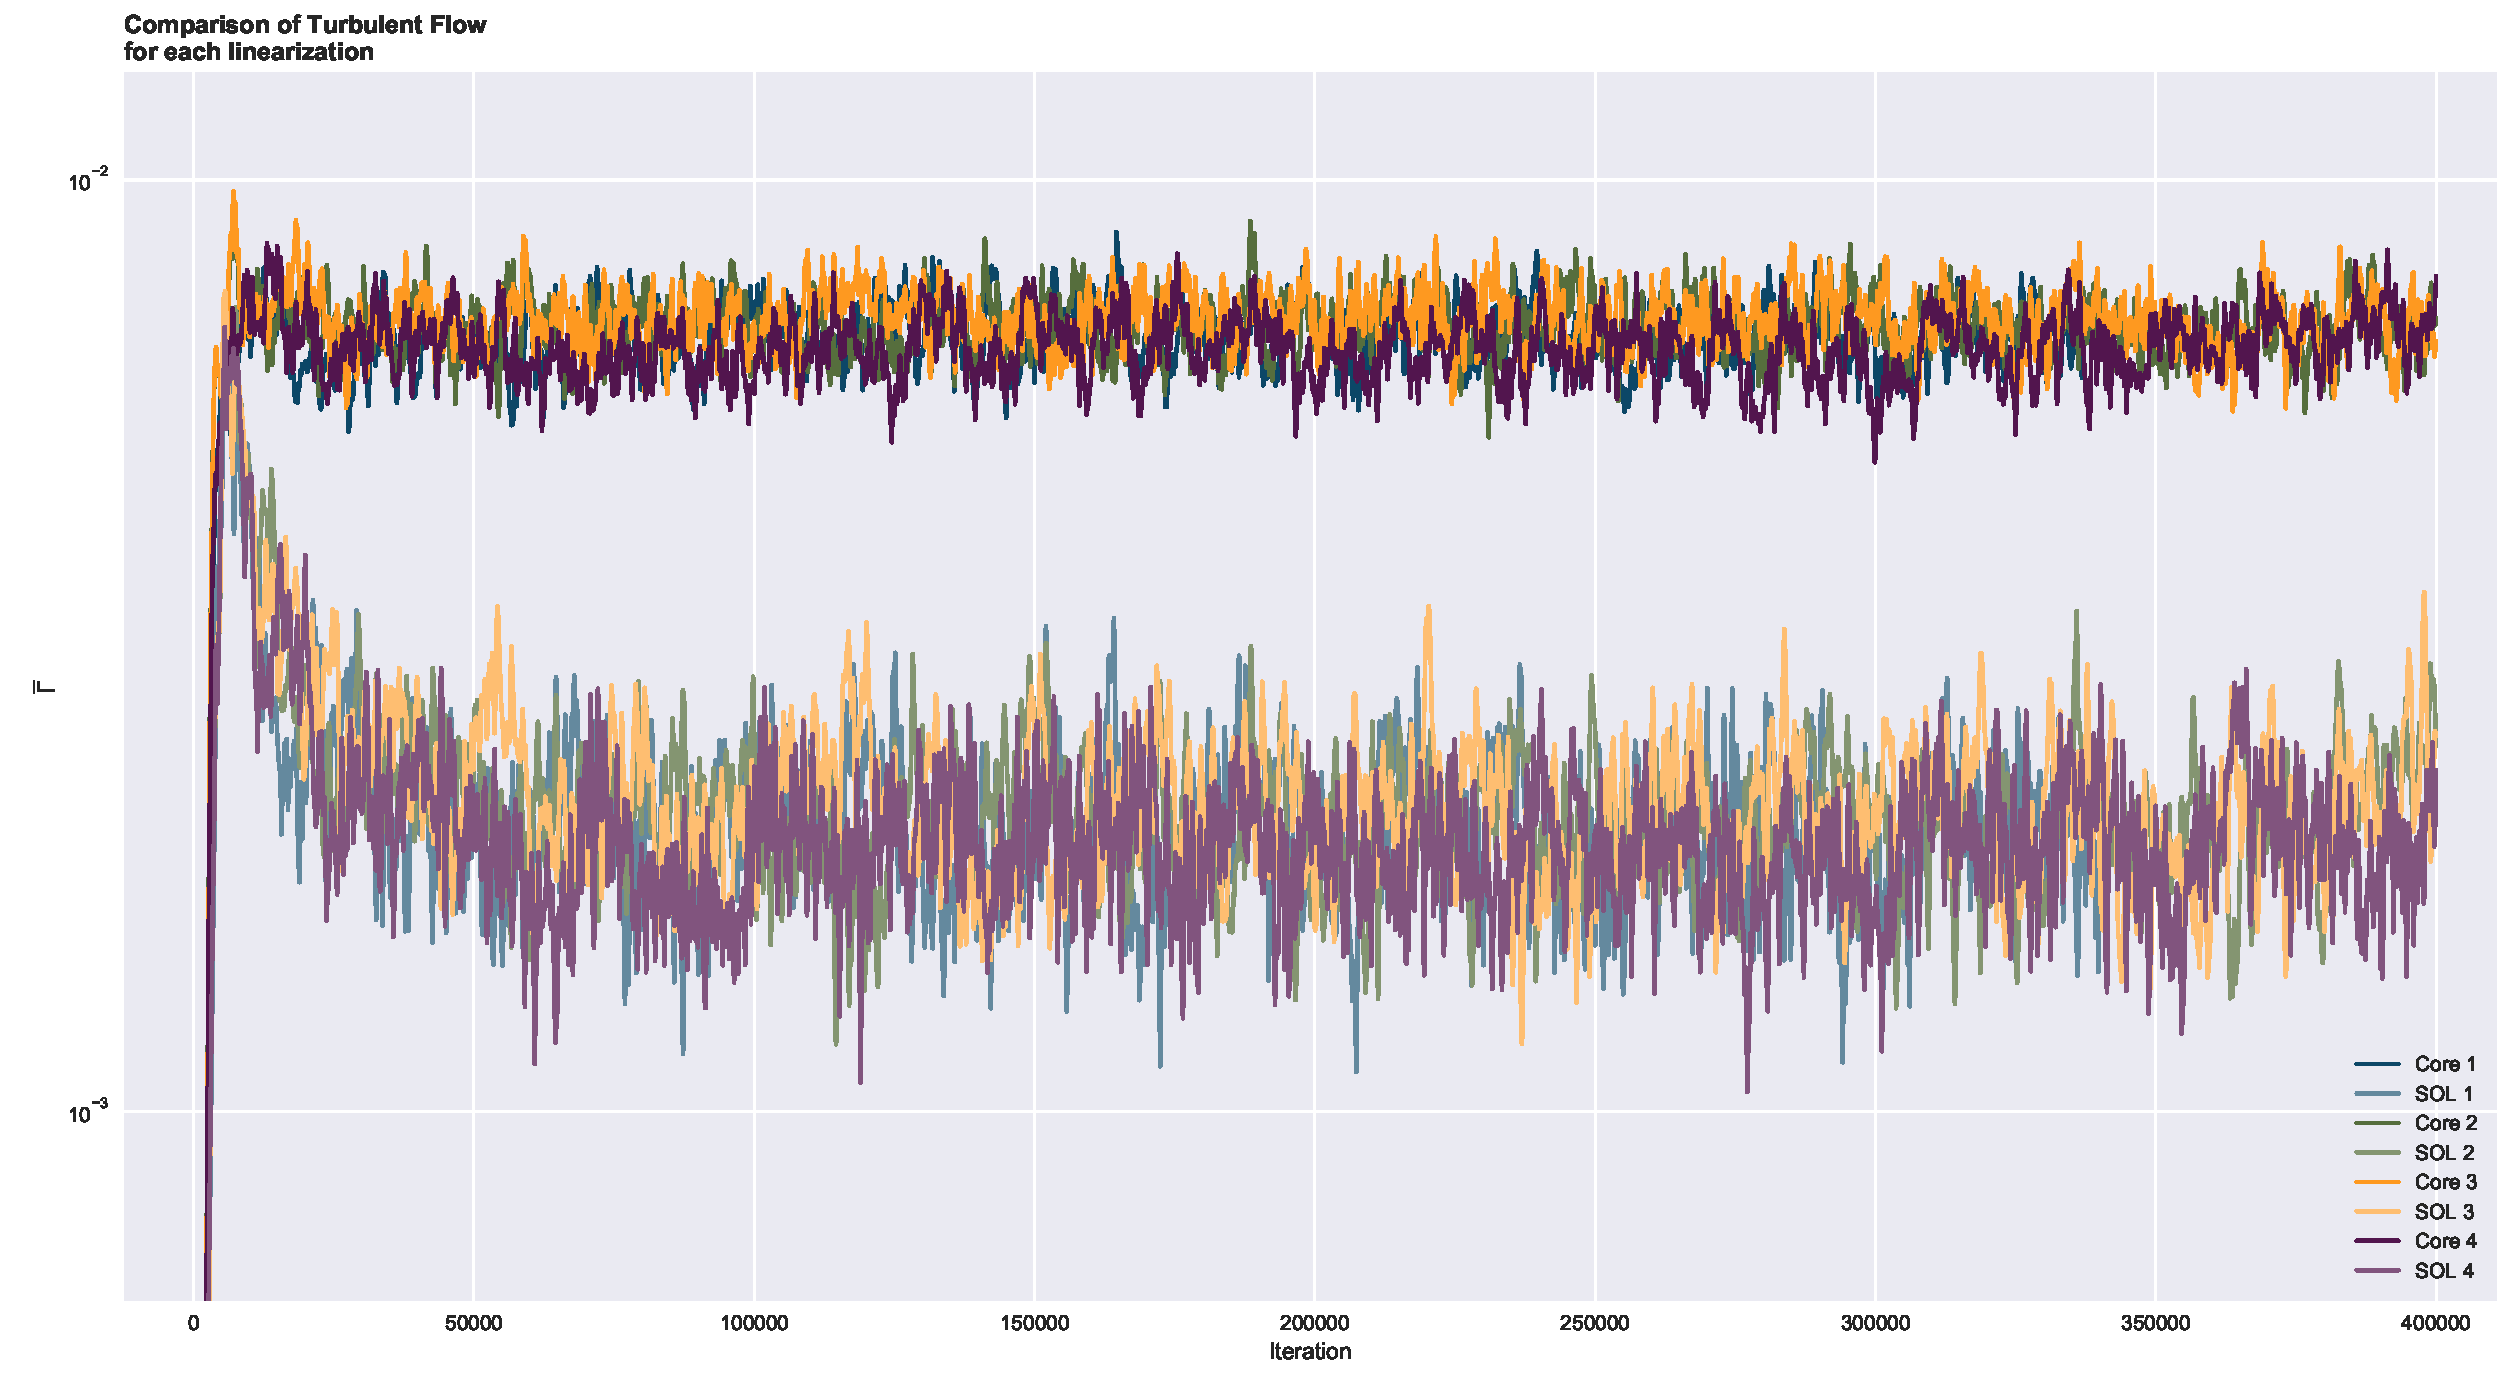
\includegraphics[width=\linewidth]{pdfs/turbulent-flow-low.pdf}
    \caption{Turbulent flow split into Core and \ac{SOL} region for each linearization. The lighter colors represent the \ac{SOL} parts.}
    \label{fig:turbulent-flow-low}
\end{figure}
\autoref{fig:turbulent-flow-low-means} shows the mean value of $\Tflow_{Core}$ and $\Tflow_{SOL}$ from 120,000 to 400,000 iterations. There may be a small indication that $\Tflow_{Core}$ is a little higher for the constant background (local model) lineraizations but considering the magnitude of fluctuations (visualized by the error bars) this seems very far fetched. 



\begin{figure}[!htbp]
    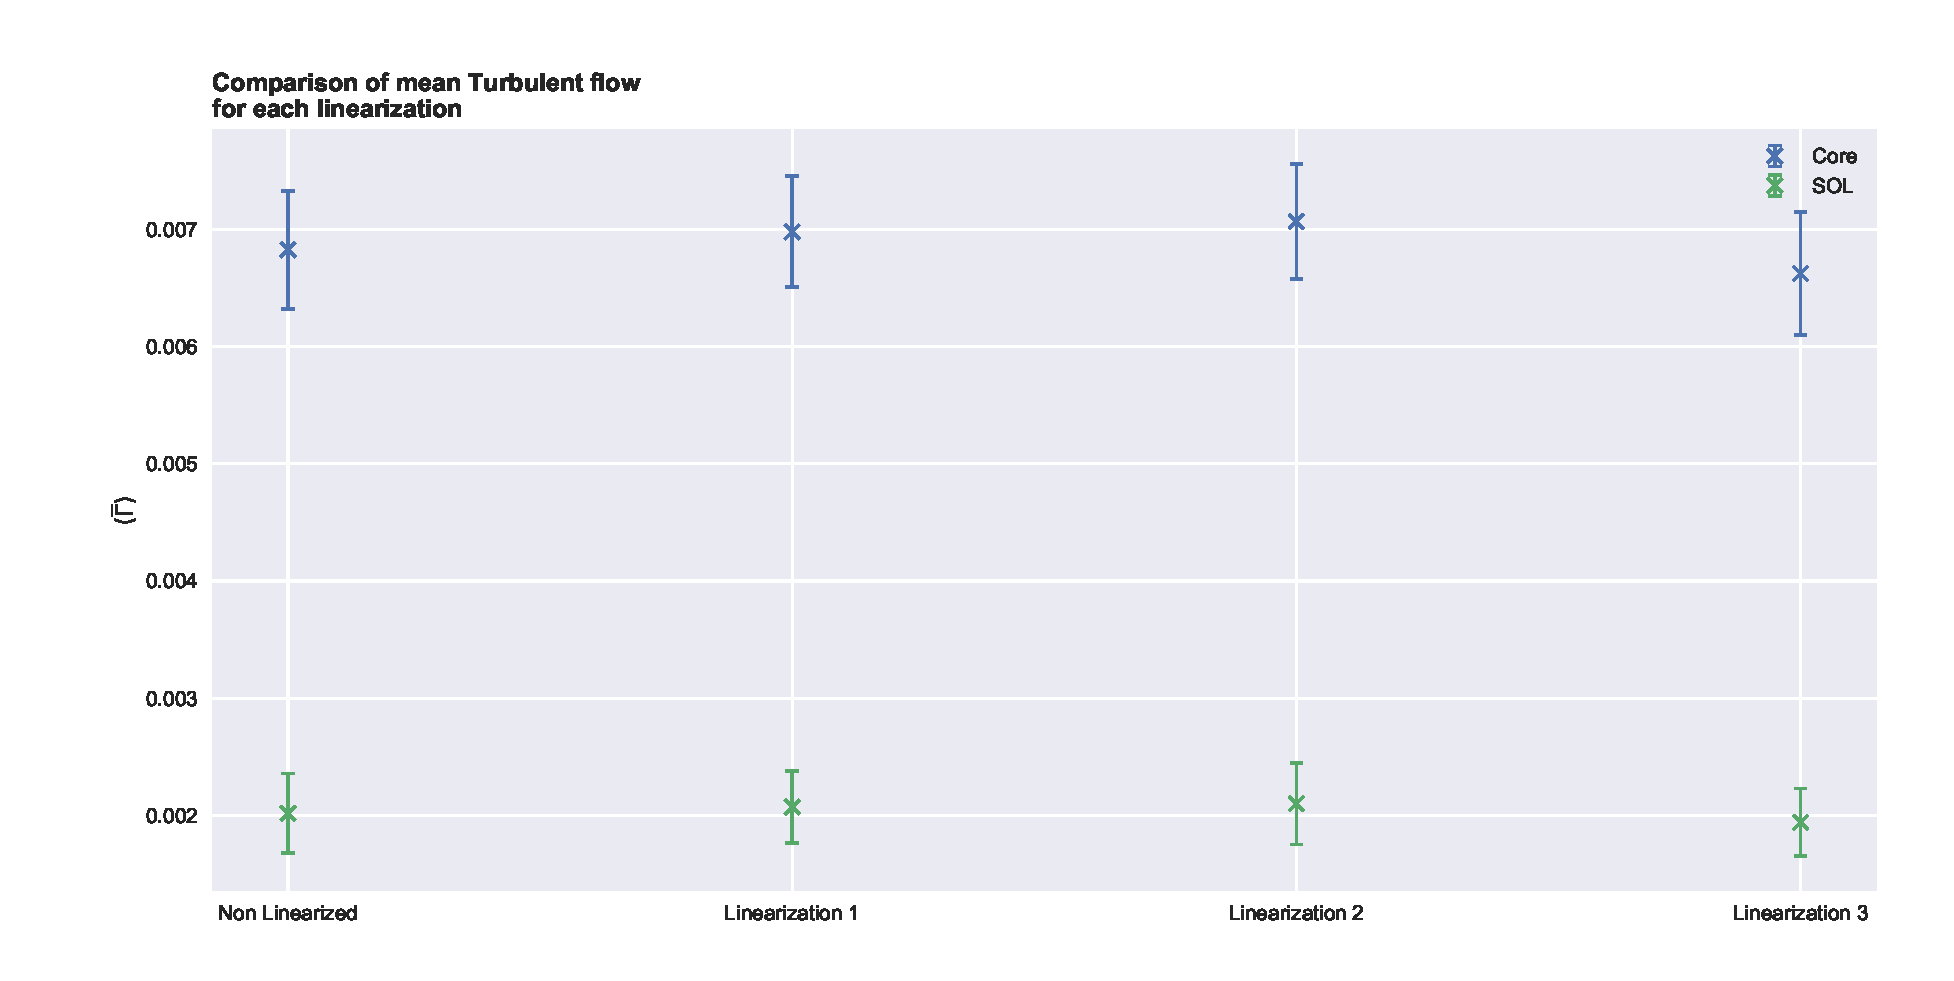
\includegraphics[width=\linewidth]{pdfs/turbulent-flow-low-means.pdf}
    \caption{Mean values of $\Tflow$ after 120,000 iterations. There is no apparent difference visible.}
    \label{fig:turbulent-flow-low-means}
\end{figure}

\section{Zonal Potential}


\begin{figure}[!htbp]
    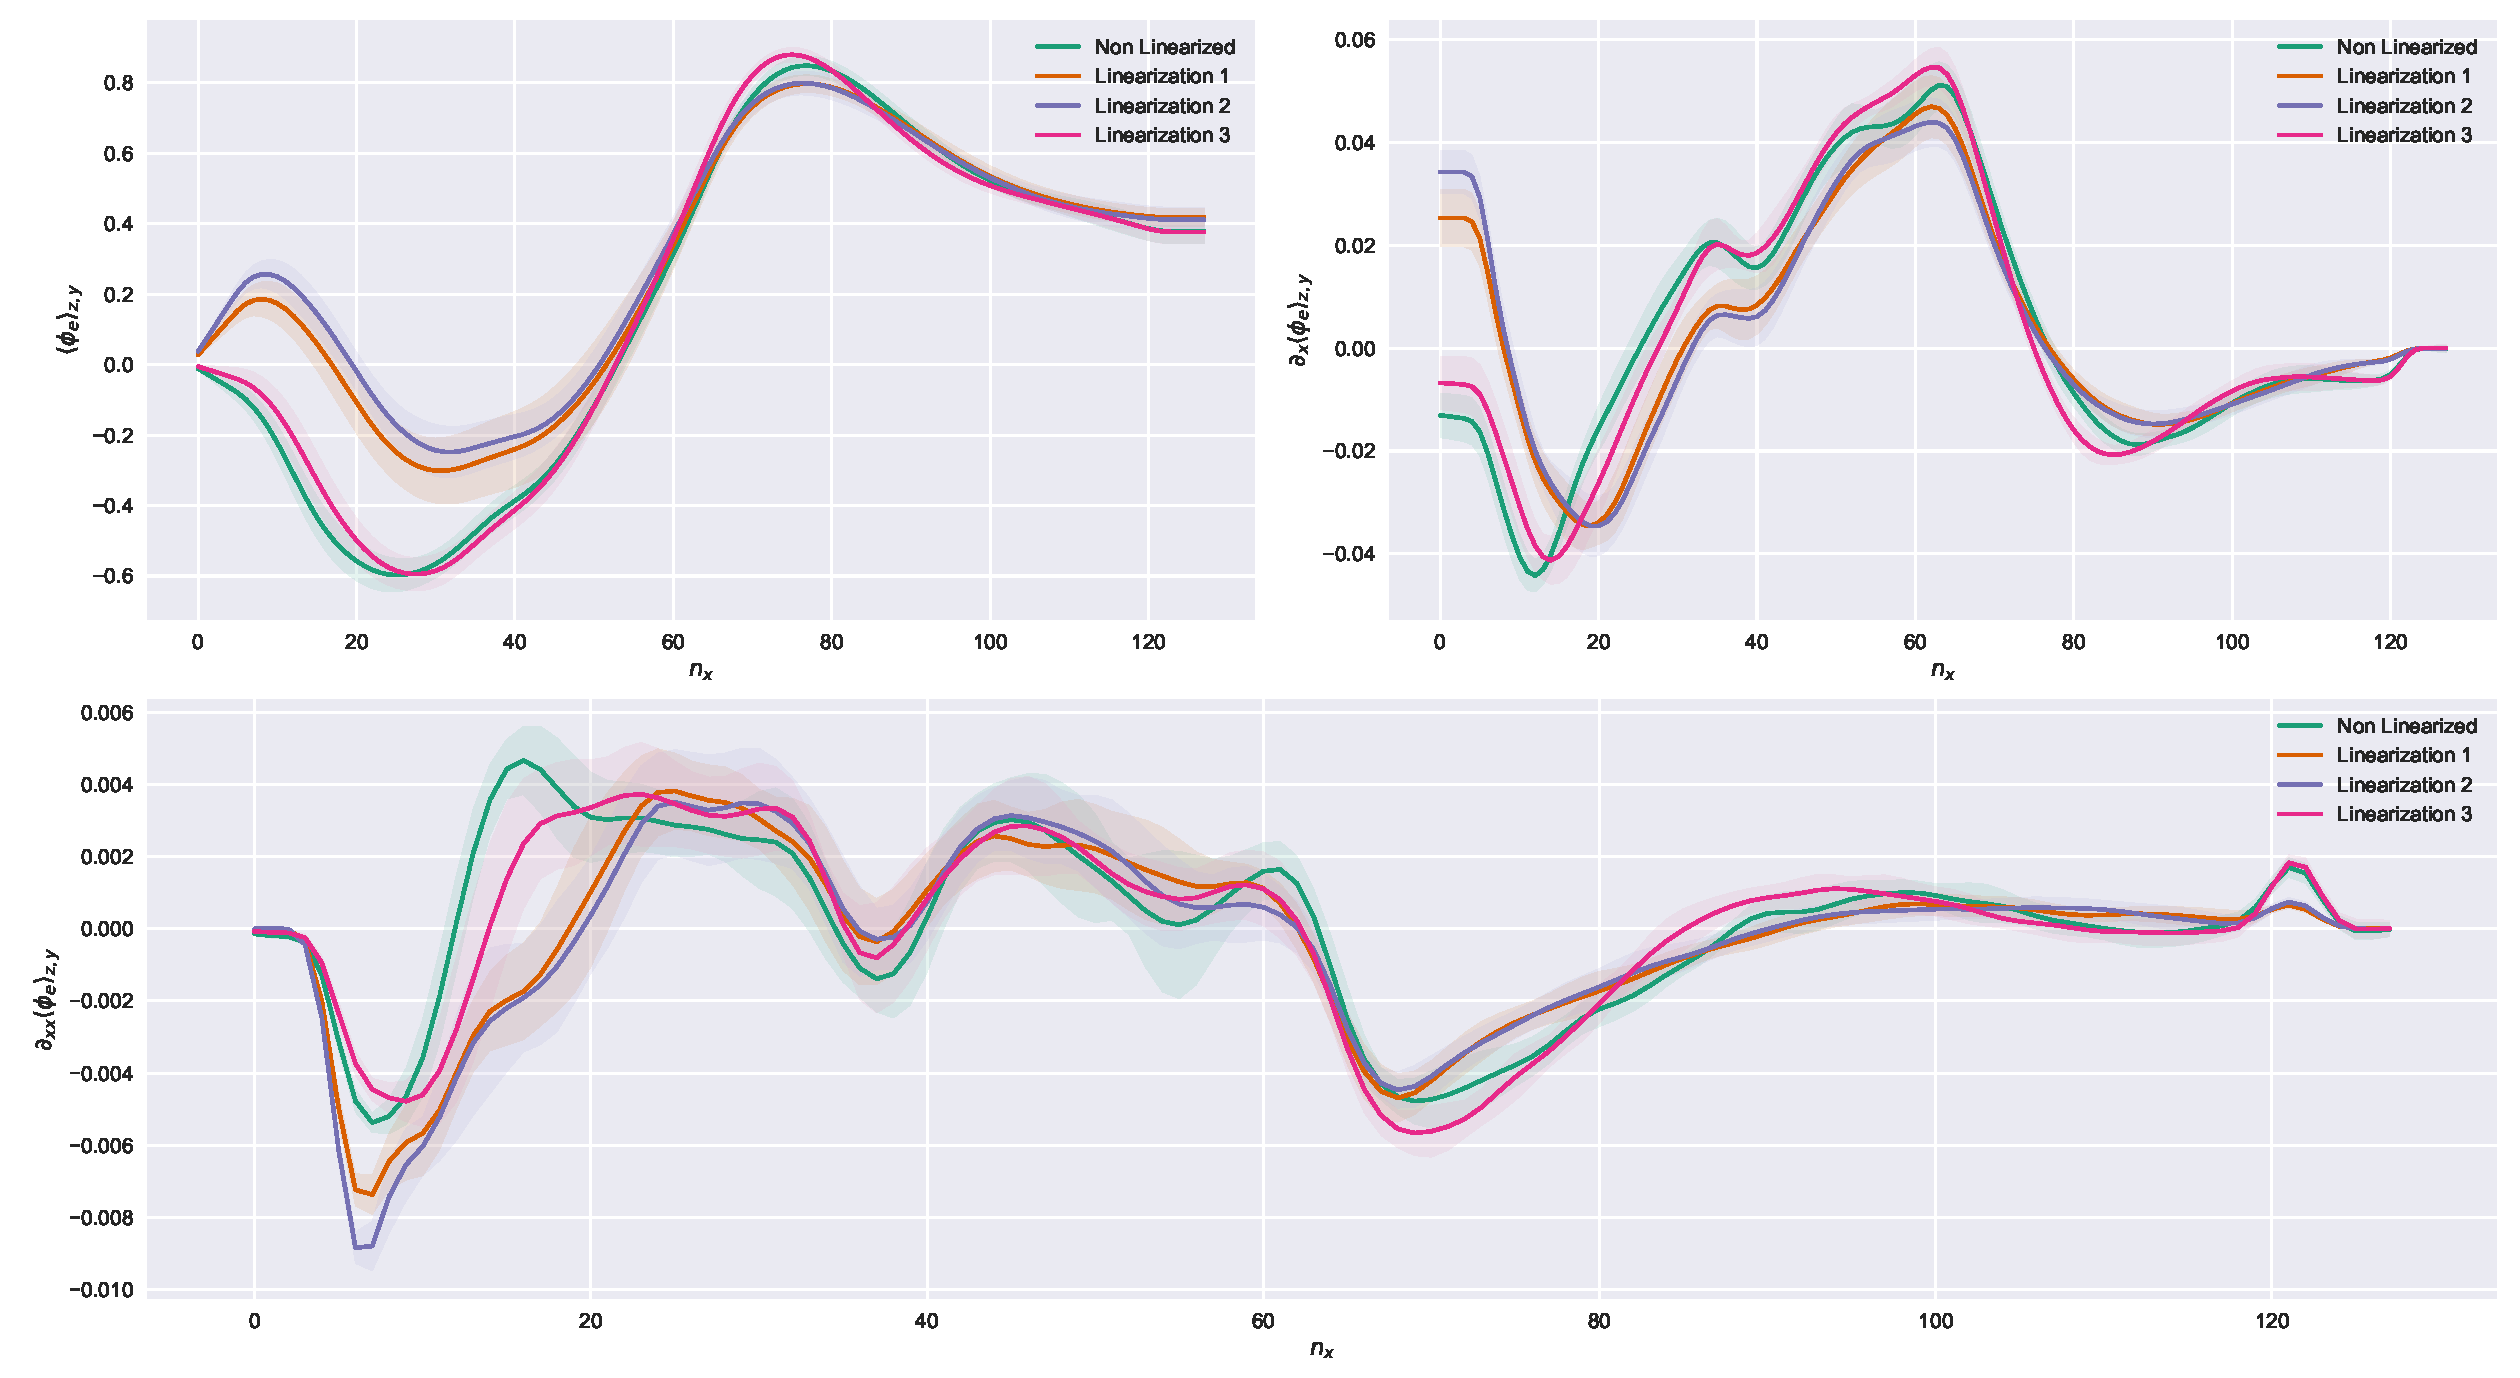
\includegraphics[width=\linewidth]{pdfs/zonal_potential_low.pdf}
    \caption{Mean values of Zonal Potential, Zonal Flow and Zonal Flow Potential of iteration 120,000-400,000}
    \label{fig:zonal-potential-low-all}
\end{figure}


\end{document}